We believe that building models of the world knowledge is a necessary step towards operating an automated kitting workstation. The proposed models include representations for non-executable information about the kitting workstation such as information about parts, kits, and trays. The description of these models includes for instance the location, orientation, and relation between components. These models are discussed in Section~\ref{owlkitting}.

Models of executable information are also produced from the system information described in the SVR. These models include actions, actions' precondition, actions' effect, and actions' failures that consist of different spatial relations. A description of these models is given in Section~\ref{owlsoap}.

Models for executable and non-executable information can be combined to generate the OWL/XML kitting \onto{init} and \onto{goal} conditions files, as described in Section~\ref{owlinitgoal}.

%+++++++++++++++++++++++++++++++++++++++++++++++++++++++++++%
\subsection{The OWL/XML Kitting Ontology}\label{owlkitting}
%+++++++++++++++++++++++++++++++++++++++++++++++++++++++++++%
In order to maintain compatibility with the IEEE working group, the \onto{Kitting} ontology has been fully defined in the Web Ontology Language (OWL)~\cite{OWLoverview}. In addition, the ontology was also fully defined in the XML schema language~\cite{Walmsley.2002}. Although the two models are conceptually identical, there are some systematic differences between the models (in addition to differences inherent in using two different languages).


\begin{itemize}
  \item The \textsf{complexType} names (i.e. class names) in XML schema have the suffix ``Type" added which is not used in OWL. This is so that the same names without the suffix can be used in XML schema language as element names without confusion.
  \item All of the XML schema \textsf{complexTypes} have a ``Name" element that is not present in OWL. It is not needed in OWL because names are assigned as a matter of course when instances of classes are created.
  \item The XML schema model has a list of ``Object" elements. This collects all of the movable objects. The OWL model does not have a corresponding list. In an OWL data file, the movable objects may appear anywhere.
  \item OWL has classes but does not have attributes; it has \textsf{ObjectProperties} and \textsf{DataProperties} instead. They may be used to model attributes. OWL Properties are global, not local to a class, so localizing each attribute to a class is done by a naming convention that includes using prefixes as described below. The prefixes are not used in XML schema.
  \item OWL supports multiple inheritances, but that has not been used in the \onto{Kitting} ontology. Except by subclass relationship, no object is in more than one class.
\end{itemize}

\begin{table}[h!t!b!]
  \caption{Excerpt of the \onto{Kitting} ontology.}
  \label{tab:kittingonto}
  \centering
  \begin{tabular}{l}
    \hline
    \class{SolidObject} \textit{PrimaryLocation} \textit{SecondaryLocation}
    \\\hline
    \hspace{5 mm}\class{Kit} \textit{Tray} \textit{DesignRef} \textit{Parts} \textit{Finished?}
    \\\hline
    \hspace{5 mm}\class{LargeBoxWithEmptyKitTrays} \textit{LargeContainer} \textit{Trays}
    \\\hline
    \hspace{5 mm}\class{LargeBoxWithKits} \textit{LargeContainer} \textit{Kits} \textit{KitDesignRef} \textit{Capacity}
    \\\hline
    \hspace{5 mm}\class{PartsTrayWithParts} \textit{PartTray}
    \\\hline
    \hspace{5 mm}\ldots
    \\\hline
    \class{DataThing}
    \\\hline
    \hspace{5 mm}\class{PhysicalLocation} \textit{RefObject}
    \\\hline
    \hspace{10 mm}\class{PoseLocation} \textit{Point} \textit{XAxis} \textit{ZAxis}
    \\\hline
    \hspace{15 mm}\class{PoseLocationIn}
    \\\hline
    \hspace{15 mm}\class{PoseLocationOn}
    \\\hline
    \hspace{10 mm}\class{RelativeLocation} \textit{Description}
    \\\hline
    \hspace{15 mm}\class{RelativeLocationIn}
    \\\hline
    \hspace{15 mm}\class{RelativeLocationOn}
    \\\hline
    \hspace{5 mm}\ldots
    \\\hline
  \end{tabular}
\end{table}

\class{SolidObject} and \class{DataThing} constitute the two top-level classes of the \onto{Kitting} ontology model, from which all other classes are derived. \class{SolidObject} models solid objects, things made of matter. The \onto{Kitting} ontology includes several subclasses of \class{SolidObject} that are formed from
components that are \class{SolidObject}. The \class{DataThing} class models data for \class{SolidObject}. Examples of subclasses for \class{SolidObject} and \class{DataThing} are represented in Table~\ref{tab:kittingonto}. Items in italics following classes are names of class attributes. Derived types inherit the attributes of the parent. Each attribute has a specific type not shown in the listing below. If an attribute type has derived types, any of the derived types may be used.

Using Table~\ref{tab:kittingonto}, an example of interaction between classes \class{SolidObject} and \class{DataThing} can be expressed as follows: Each \class{SolidObject} \class{A} has at least one \class{PhysicalLocation} (the \textit{PrimaryLocation}). A \class{PhysicalLocation} is defined by giving a reference \class{SolidObject} \class{B} (\textit{RefObject}) and information saying how the position of \class{A} is related to \class{B}. \class{PhysicalLocation} consists of two types of location which are required for the operation of the kitting workstation:
\begin{itemize}
 \item Mathematically precise locations are needed to support robot motion. The mathematical location, \class{PoseLocation}, gives the pose of the coordinate system of \class{A} in the coordinate system of \class{B}. The mathematical information consists of the location of the origin of \class{A}'s coordinate system (\textit{Point}) and the directions of its Z (\textit{ZAxis}) and X (\textit{XAxis}) axes. The mathematical location variety has subclasses representing that, in addition, \class{A} is in \class{B} (\class{PoseLocationIn}) or on \class{B} (\class{PoseLocationOn}).
\item Relative locations (class \class{RelativeLocation}), specifically the knowledge that one \class{SolidObject} is in (\class{RelativeLocationIn}) or on (\class{RelativeLocationOn}) another, are needed to support making logical plans for building kits. The subclasses of \class{RelativeLocation} are needed not only for
logical planning, but also for cases when the relative location is known, but the
mathematical information is not available.
\end{itemize}


%++++++++++++++++++++++++++++++++++++++++++++++++++++++%
\subsection{The OWL SOAP Ontology}\label{owlsoap}
%++++++++++++++++++++++++++++++++++++++++++++++++++++++%
As depicted in Figure~\ref{fig:DesignArchitecture}, the \onto{SOAP} ontology imports the \onto{Kitting} ontology and is involved in the process that generates the PDDL domain file and in the predicate evaluation process. While some concepts in the \onto{SOAP} ontology are used by both processes, other concepts are exclusive to the predicate evaluation process. We approach the description of the \onto{SOAP} ontology with a discussion on each process and the concepts used by these processes.

\subsubsection{Concepts for the PDDL Domain File Generation Process}\label{sss:domainfile}
A PDDL domain file consists of definitions of actions, predicates, and functions. Actions are ways of changing the state of the world and consist of a precondition and an effect sections. Predicates and functions constitute preconditions and effects. Predicates are used to encode Boolean state variables, while functions are used to model updates of numerical values. Introducing functions into planning makes it possible to model actions in a more compact and sometimes more natural way~\cite{FOX.JAIR.2003}. Figure~\ref{fig:put-part} shows the action \texttt{put-part} as defined in the kitting domain file.

\begin{figure}[t!h!]
\begin{minipage}{.5\paperwidth}
\begin{list}{}{\setlength{\leftmargin}{1em}}\item\small
\begin{Verbatim}[commandchars=\\\{\},fontsize=\scriptsize, numbers=left, numbersep=2pt]
(:action put-part
   :parameters(
      ?robot - Robot
      ?part - Part
      ?kit - Kit
      ?worktable - WorkTable
      ?partstray - PartsTray)
   :precondition (and
      (part-location-robot ?part ?robot)
      (robot-holds-part ?robot ?part)
      (on-worktable-kit ?worktable ?kit)
      (origin-part ?part ?partstray)
      (< (quantity-kit ?kit ?partstray)
      (capacity-kit ?kit ?partstray))
      (kit-location-worktable ?kit ?worktable))
   :effect (and
      (not (part-location-robot ?part ?robot))
      (not (robot-holds-part ?robot ?part))
      (part-not-searched)
      (not (found-part ?part ?partstray))
      (part-location-kit ?part ?kit)
      (increase (quantity-kit ?kit ?partstray) 1)
      (robot-empty ?robot))
)
\end{Verbatim}
\end{list}
\end{minipage}
\caption{PDDL action put-part.}
\label{fig:put-part}
\end{figure}

A PDDL action consists of the following sections:
\begin{enumerate}
  \item \texttt{action} (line 1): The unique name of the action comes directly after the keyword \texttt{:action}. In this example, the name of the action is \texttt{put-part}.
  \item \texttt{parameters} (lines 2--7): The parameters (start with a ? mark) that participate in this action are listed along their types. For example, line 3 can be read as ``\texttt{robot} is a parameter and is of type \texttt{Robot}''.
  \item \texttt{precondition} (lines 8--15): This section lists all the predicates (functions) that need to be true (satisfied) for the action to be carried out.
  \item \texttt{effect} (lines 16--23): This section lists all the predicates (functions) that are true (satisfied) when the action is performed.
  \item \texttt{predicate} and \texttt{function}: In Figure~\ref{fig:put-part}, the \texttt{precondition} section includes an operation between functions (lines 13--14) and the \texttt{effect} section includes one function at line 22. The other components of the precondition and the effect sections are predicates and negation of predicates (identified by the keyword \texttt{not}).
\end{enumerate}

In the \onto{SOAP} ontology, the concepts of ``Action", ``Precondition", ``Effect", ``Predicate", ``Function", and ``Parameter" are represented by the classes \class{Action}, \class{Precondition}, \class{Effect}, \class{Predicate}, \class{Function}, and \class{ParameterList}, respectively. Operations between functions (lines 13--14) that return a Boolean value are expressed in the class \class{FunctionBool}. All the aforementioned classes are subclasses of the \class{DataThing} class discussed in Section~\ref{owlkitting}.

PDDL actions have been represented in OWL with relations between classes as described below. In these descriptions, the term ``occurrence" refers to the number of times a relation between two classes can appear in the ontology. For instance, an occurrence $0\ldots\infty$ means that a relation between two classes may not appear or may appear multiple times in the ontology.

%\begin{enumerate}
%  \item Each instance of the class \class{Action} points (1 occurrence) to an instance of the class \class{ParameterList}.
%    \begin{enumerate}
%      \item Each instance of the class \class{ParameterList} points ($1\ldots\infty$ occurrences) to an instance of a class in the \texttt{Kitting} ontology. In Figure~\ref{fig:put-part}, the parameter \texttt{robot} is an instance of the class \class{Robot} which is a subclass of \class{SolidObject} in the \texttt{Kitting} ontology.
%    \end{enumerate}
%  \item Each instance of the class \class{Action} points (1 occurrence) to an instance of the class \class{Precondition}.
%    \begin{enumerate}
%      \item Each instance of the class \class{Precondition} points ($0\ldots\infty$ occurrences) to an instance of the class \class{Predicate}. A precondition can consist only of functions and has no predicates.
%	\begin{enumerate}
%	  \item Each instance of the class \class{Predicate} points ($0\ldots2$ occurrences) to an instance of  a class in the \texttt{Kitting} ontology. In most domains, including our kitting domain, predicates have a maximum of two parameters. This is the result of the definition of state variables in the SVR~\cite{BALAKIRSKY.IROS.2012}. Note that the instance of the class in the \texttt{Kitting} ontology is the same one defined in 1(a). This way assures that the predicate's parameters refer to the same parameters defined for the action.
%	\end{enumerate}
%      \item Each instance of the class \class{Precondition} points ($0\ldots\infty$ occurrences) to an instance of the class \class{Function}. A precondition can consist only of predicates and has no functions.
%	\begin{enumerate}
%	  \item Each instance of the class \class{Function} points ($1\ldots\infty$ occurrences) to an instance of a class in the \texttt{Kitting} ontology. This instance of the class in the \texttt{Kitting} ontology is the same one defined in 1(a) for the same reason described in 2(a)i.
%	\end{enumerate}
%      \item Each instance of the class \class{Precondition} points ($0\ldots\infty$ occurrences) to an instance of the class \class{FunctionBool}.
%        \begin{enumerate}
%	  \item Each instance of the class \class{FunctionBool} points (2 occurrences) to the class \class{Function} to formulate the kind of operation depicted at lines 13--14 in Figure~\ref{fig:put-part}.
%	\end{enumerate}
%    \end{enumerate}
%  \item Each instance of the class \class{Action} points (1 occurrence) to an instance of the class \class{Effect}.
%    \begin{enumerate}
%      \item The class \class{Effect} has the same relations as the ones described for the class \class{Predicate} (2(a), 2(b), and 2(c)). Note that the effect section can contain $1\ldots\infty$ occurrences of negative predicates. Negative predicates are expressed in OWL with the property assertion \texttt{owl:NegativePropertyAssertion}.
%    \end{enumerate}
%\end{enumerate}


\begin{enumerate}
  \item Each instance of the class \class{Action} is related ($1$ occurrence) to an instance of the class $\mathcal{C}$.
    \begin{enumerate}
      \item $\mathcal{C}$=\class{ParameterList}
      \item $\mathcal{C}$=\class{Precondition}
      \item $\mathcal{C}$=\class{Effect}
    \end{enumerate}
  \item Each instance of the class \class{ParameterList} is related ($1\ldots\infty$ occurrence(s)) to an instance of a class in the \onto{Kitting} ontology. In Figure~\ref{fig:put-part}, the parameter \texttt{robot} is an instance of the class \class{Robot} which is a subclass of \class{SolidObject} in the \onto{Kitting} ontology.

  \item Each instance of the class \class{Precondition} is related ($0\ldots\infty$ occurrence(s)) to an instance of the class $\mathcal{C}$.
    \begin{enumerate}
      \item $\mathcal{C}$=\class{Predicate}. A precondition can consist only of functions and has no predicates.
       \item $\mathcal{C}$=\class{Function}. A precondition can consist only of predicates and has no functions.
       \item $\mathcal{C}$=\class{FunctionBool}.
    \end{enumerate}
    \item Each instance of the class \class{Effect} is related ($x$ occurrence(s)) to an instance of the class $\mathcal{C}$.
    \begin{enumerate}
      \item $x$=$1\ldots\infty$, $\mathcal{C}$=\class{Predicate}. An effect can consist only of functions and has no predicates. Note that negative predicates are considered to be from the class \class{Predicate}. Negative predicates are expressed in OWL with the property assertion\\\texttt{owl:NegativePropertyAssertion}.
      \item $x$=$0\ldots\infty$, $\mathcal{C}$=\class{Function}. An effect can consist only of predicates and has no functions.
      \item $x$=$0\ldots\infty$, $\mathcal{C}$=\class{FunctionBool}. A precondition can consist only of predicates and has no functions.
    \end{enumerate}
  \item Each instance of the class \class{Predicate} is related ($0\ldots2$ occurrence(s)) to an instance of a class in the \onto{Kitting} ontology. In most domains, including our kitting domain, predicates have a maximum of two parameters. This is the result of the definition of state variables in the SVR~\cite{BALAKIRSKY.IROS.2012}. Note that the instance of the class in the \onto{Kitting} ontology is one of the instances defined in item 2. This way assures that the predicate's parameters refer to the same parameters defined for the action.
  \item Each instance of the class \class{Function} is related ($1\ldots\infty$ occurrence(s)) to an instance of a class in the \onto{Kitting} ontology. This instance of the class in the \onto{Kitting} ontology is one of the instances defined in item 2.
    \item Each instance of the class \class{FunctionBool} is related ($2$ occurrences) to an instance of the class \class{Function}. This is used to formulate the kind of operation depicted at lines 13--14 in Figure~\ref{fig:put-part}.
\end{enumerate}

%-------------------------------------------------------------%
\subsubsection{Concepts for Action Failure}\label{sss:failure}
%-------------------------------------------------------------%
 A failure is any change or any design or manufacturing error that renders a component, assembly, or system incapable of performing its intended function. In the knowledge driven diagram (Figure~\ref{fig:DesignArchitecture}), the \process{Predicate Evaluation} process is responsible for failure detection. An action failure consists of failure modes that can occur during the execution of a PDDL action. The steps to identify action failures in the kitting system are described in Figure~\ref{fig:algo}.

\begin{figure}[h!t!]
  \centering
  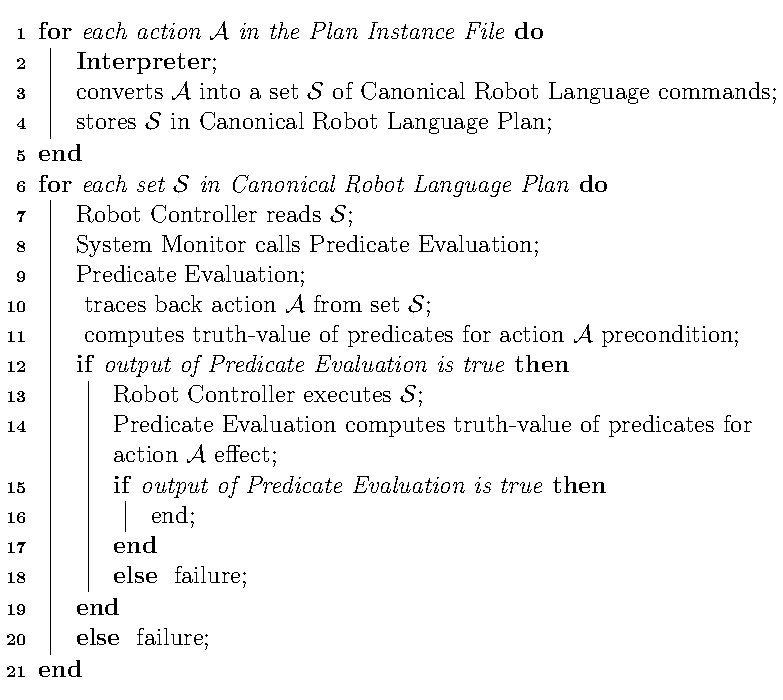
\includegraphics[width=10cm]{images/algorithm.pdf}
  \caption{Failure identification.}
  \label{fig:algo}
\end{figure}

As seen in Figure~\ref{fig:algo}, failures are identified during the execution of canonical robot commands (line 6), generated from PDDL actions (line 3) by the \process{Interpreter}. The \process{Predicate Evaluation} process outputs a Boolean value that results in a failure detection if this value is false (lines 18 and 20). Therefore, to represent failures in the \onto{SOAP} ontology, the following concepts are introduced:
\begin{itemize}
 \item ``Action'' the PDDL action for which a failure can occur.
 \item ``Failure Mode(s)'' for a PDDL action.
 \item ``Cause(s)'' of failure. Causes can be of different types, such as  components, usage conditions, human interaction, internal factors, external factors, etc.
 \item ``Predicate(s)'' responsible for generating a ``Failure Mode''.
 \item ``Effect'' of the failure.
 \item ``Severity'' of the ``Effect(s)''. Assessment of how serious the effects would be should the failure occur. Each effect is given a rank of severity ranging from 1 (minor) to 10 (very high). The severity rank is used to trigger the appropriate contingency plan.
 \item ``Probability of Occurrence'': an estimate number of frequencies (based on experience) that a failure will occur for a specific action.
\end{itemize}

Table~\ref{tab:putpartfailure} shows an example of failure modes associated to the PDDL action \textit{put-part}(\stvar{robot},\stvar{part},\stvar{kit},\stvar{worktable},\stvar{partstray}) which is defined as ``The Robot \stvar{robot} puts the Part \stvar{part} in the Kit \stvar{kit}''.
%previously presented in Figure~\ref{fig:put-part}.

%%%%%%%%%%%%%%%%%%%%%%%%%%%%%%%%%%%%
%%%%%%%%%%% put-part %%%%%%%%%%%
%%%%%%%%%%%%%%%%%%%%%%%%%%%%%%%%%%%%
\begin{table}[h!t!]
  %\centering
  \caption{Failure modes for the PDDL action \textit{put-part}.}
  \label{tab:putpartfailure}
  \scalebox{0.6}{
  \begin{tabular}{|l|l|l|l|c|c|c|}
    \hline
    \multicolumn{1}{|c|}{\begin{sideways}Action\end{sideways}} &
    \multicolumn{1}{c|}{\begin{sideways}Failure Mode(s) \,\end{sideways}} &
    \multicolumn{1}{c|}{\begin{sideways}Cause(s) \,\end{sideways}} &
    \multicolumn{1}{c|}{\begin{sideways}Effect(s) \,\end{sideways}} &
    \multicolumn{1}{c|}{\begin{sideways}Severity \,\end{sideways}} &
    \multicolumn{1}{c|}{\begin{sideways}Occurrence (\%) \,\end{sideways}} &
    \multicolumn{1}{c|}{\begin{sideways}Predicate(s) \,\end{sideways}} \\
    \hline
    
    \multirow{5}{*}{\textit{\small{put-part}}} & 
    \multirow{2}{*}{\stvar{part} falls off of the end effector} & 
    \multirow{2}{*}{end effector hardware issues} & 
    downtime & %\stvar{endeffector} replacement &  
    9 &
    \multirow{2}{*}{60} & 
    \small {\textsf{part-location-robot}}\\\cline{4-5}
    
     & 
     & 
     & 
    \stvar{part} damage & %\stvar{endeffector} replacement &  
    5 &
     & 
    \small {\textsf{robot-holds-part}}\\\cline{2-7}
    
     & 
     \multirow{3}{*}{\stvar{part} not released at all}& 
     end effector hardware issues & 
     downtime & 
     9 &
     \multirow{3}{*}{8} & 
     $\neg$(\small{\textsf{part-location-robot}})\\\cline{3-5}
     
     & 
     & 
     \multirow{2}{*}{wrong/inexistant canonical command} & 
     \multirow{2}{*}{downtime} & 
     \multirow{2}{*}{7} &
      & 
     $\neg$(\small{\textsf{robot-holds-part}})\\
%    
     & 
     & 
     & 
     & 
     &
     & 
     \small {\textsf{robot-empty}}\\\hline

\end{tabular}
}
\end{table}
The column \textit{Predicate(s)} shows the predicates from the action \textit{put-part} that can activate the corresponding failure mode (column \textit{Failure Mode(s)}) if their truth-value is evaluated to false.

The representation of action failures in the \onto{SOAP} ontology includes the concepts defined earlier in this section, i.e., ``Action'', ``Failure Mode'', ``Cause'', ``Predicate'', ``Effect'', ``Severity'' and ``Probability of Occurrence''. The concepts of ``Action'' and ``Predicate'' have been discussed in earlier sections and are represented by the OWL classes \class{Action} and \class{Predicate}, respectively. The concepts of ``Failure Mode'', ``Effect'', and ``Severity'' are represented by the OWL classes \class{FailureMode}, \class{FailureEffect}, and \class{FailureSeverity}, respectively. The concepts of ``Cause'' and ``Probability of Occurence'' are represented as \texttt{owl:DataProperty}. The description of action failures in the \onto{SOAP} ontology is given below.

\begin{enumerate}
 \item \class{Action} has $1\ldots\infty$ \textit{hasFailureMode} relation(s) with \class{FailureMode}.
 \item \class{FailureMode} has $1$ \textit{hasCause} \texttt{owl:DataProperty}.
 \item \class{FailureMode} has $1$ \textit{hasOccurrence} \texttt{owl:DataProperty}.
 \item \class{FailureMode} has $1\ldots\infty$ \textit{hasFailureEffect} relation(s) with \class{FailureEffect}.
 \item \class{FailureMode} has $1\ldots\infty$ \textit{hasFailurePredicate} relation(s) with \class{Predicate}.
 \item \class{FailureEffect} has $1$ \textit{hasFailureSeverity} relation(s) with \class{FailureSeverity}.
  \item \class{FailureEffect} has $1$ \textit{hasEffectDescription} relation(s) \texttt{owl:DataProperty}.
\end{enumerate}




% \begin{algorithm}[t]
% \SetLine
% \For{each action $\mathcal{A}$ in the Plan Instance File}{
%   \process{Interpreter}\;
%   converts $\mathcal{A}$ into a set $\mathcal{S}$ of Canonical Robot Language commands\;
%   stores $\mathcal{S}$ in Canonical Robot Language Plan\;
% }
% \For{each set $\mathcal{S}$ in Canonical Robot Language Plan}{
%   Robot Controller reads $\mathcal{S}$\;
%   System Monitor calls Predicate Evaluation\;
%   Predicate Evaluation\; 
%   \ traces back action $\mathcal{A}$ from set $\mathcal{S}$\;
%   \ computes truth-value of predicates for action $\mathcal{A}$ precondition\;
%   \If{output of Predicate Evaluation is true}{
%     Robot Controller executes $\mathcal{S}$\;
%     Predicate Evaluation computes truth-value of predicates for action $\mathcal{A}$ effect\;
%      \If{output of Predicate Evaluation is true}{end\;     
%     }
%     \lElse{
%     failure\;
%   }
%   }
%   \lElse{
%     failure\;
%   }
% }
% \caption{How to write algorithms}
% \label{fig:algo}
% \end{algorithm}
 
 
 
 
%  In the knowledge driven diagram depicted in Figure~\ref{fig:DesignArchitecture}, the \process{Interpreter} converts plan actions into canonical robot commands. A single action usually consists of numerous canonical robot commands. The following steps describe how each process is called and how action failures are identified.
% \begin{enumerate}
%  \item The \process{Robot Controller} stores the set of canonical robot commands associated to the first plan action in a queue.
%  \item the \process{System Monitor} triggers the \process{Predicate Evaluation} process to compute the truth-value of the predicates that constitute the precondition section of this action.
%  \item If the \process{Predicate Evaluation} process returns true, i.e., all the predicates in the precondition section are true:
%  \begin{enumerate}
%  \item The \process{Robot Controller} executes the robot commands previously stored in its queue.
%  \item Once all the canonical robot commands have been carried out by the robot, the \process{System Monitor} once again triggers the \process{Predicate Evaluation} process to compute the truth-value of the predicates that constitute the effect section of this PDDL action.
% \end{enumerate}
% \end{enumerate}

 %We are using an approach based on the Failure Modes and Effects Analysis (FMEA) method~\cite{NANNIKAR.ICTBM.2012} to describe failure modes in our kitting system. The main goal of the FMEA is to connect failure modes as closely as possible with the source and thus enables the identification of the origin of the risk. The FMEA also allows the selection of ways to detect the occurrence of a particular failure and/or to find options to stop or lessen the effects of this failure.
%FMEA is a systematic method of identifying and preventing system, product and process problems before they occur and addresses reliability during the early stages of design. Analyzing failure modes in the design process allows calls of contingency plans when failures occur during the process. Section X describes the different steps adopted by the FMEA to identify failure modes and Section Y shows the approach we have taken to represent failure modes in the \onto{SOAP} ontology.

% \begin{figure}[h!t!]
% \centering
% 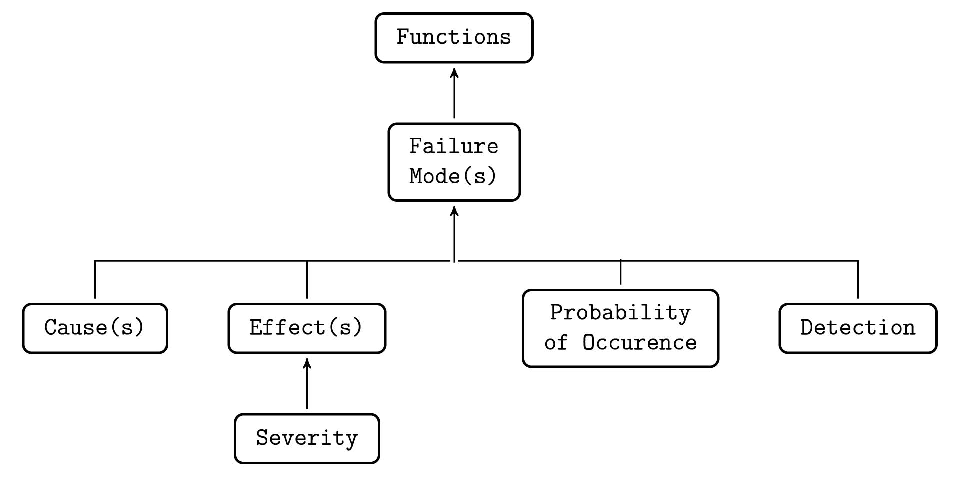
\includegraphics[width=12cm]{images/ActionFailures.pdf}
% \caption{The FMEA Process.}
% \label{fig:ActionFailures}
% %\end{center}
% \end{figure}


% The different tasks to represent action failures using the FMEA process are shown in Figure~\ref{fig:ActionFailures}. Each block portrayed in the diagram is described below.
% 
%  \begin{itemize}
%    \item \texttt{Functions}: The specific behavior or attribute intended by design. In our kitting system, FMEA functions are represented by PDDL actions.
%    \item \texttt{Failure Modes}: Description of everything that can go wrong for a particular function.
%    \item \texttt{Cause(s)}: List of possible causes that triggered a specific failure. Causes can be of different types, such as  components, usage conditions, human interaction, internal factors, external factors, etc.
%    \item \texttt{Effect(s)}: Description of consequences of a system. A typical failure mode may have several effects.
%    \item \texttt{Severity}: Assessment of how serious the effects would be should the failure occur. Each effect is given a rank of severity ranging from 1 (minor) to 10 (very high). An example of severity ranking criteria is given in Table~\ref{tab:severityrankingcriteria}.
%    \item \texttt{Probability of Occurrence}: The probability of occurrence is an estimate number of frequencies (based on experience) that a failure will occur for a specific function.
%    \item \texttt{Detection}: Assessment of the probability that the failure mode will be detected before the impact
% of the failure to the system or process being evaluated is detected.
% \item \texttt{Predicate(s)}: We have adapted the FMEA process to our system by including the predicate(s) responsible for a failure mode. As discussed in Section~\ref{}, the \process{Predicate Evaluation} process computes the truth-value for a predicate and returns a Boolean. An action failure is identified when the truth-value of one or more predicates that constitute this action returns false.
%  \end{itemize}
% 
% \begin{table}[!t!h]
% \centering
% \caption{Severity Ranking Criteria for Kitting.}
% \label{tab:severityrankingcriteria}
% \scalebox{1}{
% \begin{tabular}{lc}
% \hline
% \textbf{Rank} & \textbf{Description}\tabularnewline
% \hline
% \tabularnewline
% 1--2 &
% \begin{minipage}[m]{0.8\columnwidth}%
% \textbf{The final kit is built} but contains failures of minor nature, undetectable by the customer. An example of minor failure is a small scratch on the paint of a component.
% \end{minipage}\tabularnewline
% \\\hline
% \tabularnewline
% 6--7 &
% \begin{minipage}[m]{0.8\columnwidth}%
% \textbf{The final kit is built} but contains slight deterioration of component or leads to slight deterioration of the system performance. For example, the locations of two components in the kit have been switched during the kit building process.
% \end{minipage}\tabularnewline
% \\\hline
% \tabularnewline
% 8--9 &
% \begin{minipage}[m]{0.8\columnwidth}%
% \textbf{The final kit is not built} and the failure will result deterioration of the system performance. For example, a supply box runs out of components that results in downtime in the process.
% \end{minipage}\tabularnewline
% \\\hline
% \tabularnewline
% 10 &
% \begin{minipage}[m]{0.8\columnwidth}%
% \textbf{The final kit is not built} and the failure will cause non-functionality of system. The origin can be a hardware or software failure.
% \end{minipage}\tabularnewline
% \\\hline
% \end{tabular}
% }
% \end{table}
% 
% Table~\ref{} shows an example of failure modes associated to the PDDL action \textit{put-part}, previously discussed in Section~\ref{sss:domainfile} and presented in Figure~\ref{fig:put-part}.
% 
% 
% %%%%%%%%%%%%%%%%%%%%%%%%%%%%%%%%%%%%
% %%%%%%%%%%% put-kittray %%%%%%%%%%%
% %%%%%%%%%%%%%%%%%%%%%%%%%%%%%%%%%%%%
% \begin{table}[h!t!]
% %\centering
% \label{tab:occurencerankingcriteria}
% \scalebox{0.45}{
% \begin{tabular}{|l|l|l|l|l|l|l|l|}
% \hline
% \multicolumn{1}{|c|}{
% \begin{sideways}
% Function
% \end{sideways}}&
% \multicolumn{1}{c|}{
% \begin{sideways}
% Failure Mode(s) \,
% \end{sideways}}&
% \multicolumn{1}{c|}{
% \begin{sideways}
% Cause(s) \,
% \end{sideways}}&
% \multicolumn{1}{c|}{
% \begin{sideways}
% Effect(s) \,
% \end{sideways}}&
% \multicolumn{1}{c|}{
% \begin{sideways}
% Severity \,
% \end{sideways}}&
% \multicolumn{1}{c|}{
% \begin{sideways}
% Occurrence (\%) \,
% \end{sideways}}&
% \multicolumn{1}{c|}{
% \begin{sideways}
% Detection (\%)\,
% \end{sideways}}&
% \multicolumn{1}{c|}{
% \begin{sideways}
% Predicate(s) \,
% \end{sideways}}
%  \\\hline
% \multirow{4}{*}{\textit{\small{put-part}}} & \stvar{part} falls off of \stvar{robot}'s \stvar{endeffector} & \stvar{endeffector} hardware issues. & downtime due to end effector replacement & 8 & 20 & 5& \small {\textsf{part-location-robot}}\\\cline{2-8}
% & \stvar{part} put at the wrong location in \stvar{kit} & wrong information in the MySQL database & downtime due to end effector replacement & 8 & 20 & 5& \small {\textsf{part-location-robot}}\\\cline{2-8}
% & \multirow{2}{*}{\stvar{part} stays in \stvar{endeffector}} & hardware issues & downtime due to end effector replacement & 8 & 20 & 5& \small {\textsf{part-location-robot}}\\\cline{3-8}
% & & software: release command not given to \stvar{robot} & & &  & & \small {\textsf{part-location-robot}}\\\cline{2-8}


% \end{tabular}
% }
% \caption{Failure modes for the PDDL action \textit{put-part}.}
% \end{table}
% 
% Based on Figure~\ref{} and Table~\ref{}, we have taken the following approach to represent action failures in the \onto{SOAP} ontology.

% 
% In the knowledge driven diagram depicted in Figure~\ref{fig:DesignArchitecture}, failures are identified when the ouput of the \process{Predicate Evaluation} process returns false, i.e., when a predicate is not true. 
% 
% 
% In the knowledge driven diagram depicted in Figure~\ref{fig:DesignArchitecture}, the \process{Interpreter} converts PDDL actions in the plan instance file into canonical robot commands where a single PDDL action consists of multiple canonical robot commands. The following steps describe how each process is called and how action failures are identified.
% \begin{enumerate}
%  \item The \process{Robot Controller} stores the set of canonical robot commands for the first PDDL action in a queue.
%  \item the \process{System Monitor} triggers the \process{Predicate Evaluation} process to compute the truth-value of the predicates that constitute the precondition section of this PDDL action.
%  \item If the \process{Predicate Evaluation} process returns true, i.e., all the predicates in the precondition section are true:
%  \begin{enumerate}
%  \item The \process{Robot Controller} executes the robot commands previously stored in its queue.
%  \item Once all the canonical robot commands have been carried out by the robot, the \process{System Monitor} once again triggers the \process{Predicate Evaluation} process to compute the truth-value of the predicates that constitute the effect section of this PDDL action.
% \end{enumerate}
% \end{enumerate}
% 
% If the the \process{Predicate Evaluation} process is true, the \process{Robot Controller} queues the set of canonical robot commands associated to the next PDDL action. If, the \process{Predicate Evaluation} process returned false
% 
% To be more specific, the truth-value of all the predicates of the precondition section in the PDDL action are computed before the \process{Robot Controller} executes the set of canonical robot commands for this action. 
% 
% Before performing a set of canonical robot commands, the \process{Robot Controller} process calls the \process{System Monitor} process to start the \process{Predicate Evaluation} process. 
% 
% 
% The predicate evaluation process is called during the execution of robot commands (defined in the Robot Language) by the robot. In our system, one PDDL action generates multiple of these commands. Before the robot executes these commands, the predicates that constitute the precondition section for the original PDDL action are evaluated. In the same way, once the set of robot commands has been carried out by the robot, the predicates part of the effect section for the original PDDL action are evaluated. In our system, we use the concept of ``Spatial Relations'' to evaluate these predicates.
% 
% Our kitting system checks for failures during the execution of robot commands by the robot controller (\textbf{Act} level in Figure~\ref{fig:DesignArchitecture}). As mentioned in Section(), the Interpreter process converts PDDL actions in the plan instance file into a set of canonical robot commands that are written in the canonical robot command language plan. This plan file is fed to the robot controller that successively executes each robot command. Before a set of robot commands is carried out by the robot controller, the system monitor invokes the \process{Predicate Evaluation} process to
% 
% 
% the execution of the plan. More precisely, before and after an action is carried out. Before an action is carried out, the predicates part of this action's precondition are verified. Once the action has been executed by the robot, the predicates part of this action's effect are also verified. More information on the methodology used to verify predicates can be found in Section~\ref{task3}. The rest of this section is built as follows: Section~\ref{ss:descriptionfailures} describes failure modes for a kitting system and Section~\ref{ss:failurespredicates} details the predicates where these failure modes can be identified.

%-------------------------------------------------------------%
\subsubsection{Concepts for the Predicate Evaluation Process}
%-------------------------------------------------------------%
As seen in Section~\ref{sss:failure}, the \process{Predicate Evaluation} process is called by the \process{System Monitor} process to check the truth-value of a predicate. The output of this process is a Boolean that is redirected back to the \process{System Monitor}. We have implemented the concept of ``Spatial Relations'' in the \onto{SOAP} ontology to be able to compute the truth-value of a predicate.

``Spatial Relations'' are represented as subclasses of the \class{RelativeLocation} class which is a subtype of the \class{PhysicalLocation} (see Table~\ref{tab:kittingonto}). There are three types of spatial relations, each represented in a separate class as described below:
\begin{itemize}
 \item \class{RCC8\_Relation}: RCC8~\cite{Wolter.KR.2000} is a well-known and cited approach for representing the relationship between two regions in Euclidean space or in a topological space. Based on the definition of RCC8, the class \class{RCC8\_Relation} consists of eight possible relations, including Tangential Proper Part (TPP), Non-Tangential Proper Part(NTPP), Disconnected (DC), Tangential Proper Part Inverse (TPPi), Non-Tangential Proper Part Inverse (NTPPi), Externally Connected (EC), Equal (EQ), and Partially Overlapping (PO). In order to represent these relations in all three dimensions for the kitting domain, we have extended RCC8 to a three-dimensions space by applying it along all three planes (x-y, x-z, y-z) and by including cardinal direction relations ``+'' and ``-''~\cite{SCHLENOFF.ECDRM.2012}. In the ontology, RCC8 relations and cardinal direction relations are represented as subclasses of the class \class{RCC8\_Relation}. Examples of such classes are \class{X-DC}, \class{X-EC}, \class{X-Minus}, and \class{X-Plus}.

 \item \class{Intermediate\_State\_Relation}: These are intermediate level state relations that can be inferred from the combination of RCC8 and cardinal direction relations. For  instance, the intermediate state relation \textbf{Contained-In} is used to describe object \textit{obj1} completely inside object \textit{obj2} and is represented with the following combination of RCC8 relations:
\begin{gather}
\textbf{Contained-In}(\textit{obj1}, \textit{obj2}) \rightarrow   \notag\\
(\texttt{x-TPP}(\textit{obj1}, \textit{obj2}) \vee \texttt{x-NTPP}(\textit{obj1}, \textit{obj2})) \wedge \notag\\
(\texttt{y-TPP}(\textit{obj1}, \textit{obj2}) \vee \texttt{y-NTPP}(\textit{obj1}, \textit{obj2})) \wedge \notag\\
(\texttt{z-TPP}(\textit{obj1}, \textit{obj2}) \vee \texttt{z-NTPP}(\textit{obj1}, \textit{obj2}))\notag
\end{gather}
In the ontology, intermediate state relations are represented with the OWL built-in property \texttt{owl:equivalentClass} that links the description of the class \class{Intermediate\_State\_Relation} to a logical expression based on RCC8 relations from the class \class{RCC8\_Relation}.
 \item \class{Predicate}: The representation of predicates has been illustrated in Section~\ref{sss:domainfile}. In this section we discuss how the class \class{Predicate} has been extended to include the concept of ``Spatial Relation''. The truth-value of predicates can be determined through the logical combination of intermediate state relations. The predicate \class{kit-location-lbwk}(\textit{kit}, \textit{lbwk}) is true if and only if the location of the kit \textit{kit} is in the large box with kits \textit{lbwk}. This predicate can be described using the following combination of intermediate state relations:
\begin{gather}
\textsf{kit-location-lbwk}(\textit{kit}, \textit{lbwk}) \rightarrow   \notag\\
\textbf{In-Contact-With}(\textit{kit}, \textit{lbwk}) \wedge \notag\\
\textbf{Contained-In}(\textit{kit}, \textit{lbwk}) \notag
\end{gather}
As with state relations, the truth-value of predicates is captured in the ontology using the \texttt{owl:equivalentClass} property that links the description of the class \class{Predicate} to the logical combination of intermediate state relations from the class \class{Intermediate\_State\_Relation}.

As seen in Section~\ref{sss:domainfile}, a predicate can have a maximum of two parameters. In the case where a predicate has two parameters, the parameters are passed to the intermediate state relations defined for the predicate, and are in turn passed to the RCC8 relations were the truth-value of these relations are computed. In the case the predicate has only one parameter, the truth-value of intermediate state relations, and by inference, the truth-value of RCC8 relations will be tested with this parameter and with every object in the environment in lieu of the second parameter. Our kitting domain consists of only one predicate that has no parameters. This predicate is used as a flag in order to force some actions to come before others during the formulation of the plan. Predicates of this nature are not treated in the concept of ``Spatial Relation''.
\end{itemize}



%+++++++++++++++++++++++++++++++++++++++++++++++++++++++++++++++++++++++++++++++++%
\subsection{The OWL/XML Kitting Init and Goal Conditions File} \label{owlinitgoal}
%+++++++++++++++++++++++++++++++++++++++++++++++++++++++++++++++++++++++++++++++++%
The OWL/XML kitting \onto{init} and \onto{goal} conditions files are used to build the PDDL problem file. This section first describes how a PDDL problem file is structured and then reviews the classes used in the different ontologies to build the PDDL problem file.

%-------------------------------------------------%
\subsubsection{Structure of a PDDL Problem File}
%-------------------------------------------------%
Figure~\ref{fig:problem} is a fragment of the problem file generated for our kitting system but it displays all the necessary components that constitute a PDDL problem file.

\begin{figure}[t!h!]
\begin{minipage}{.7\paperwidth}
\begin{list}{}{\setlength{\leftmargin}{1em}}\item\small
\begin{Verbatim}[commandchars=\\\{\},fontsize=\scriptsize, numbers=left, numbersep=2pt]
(define (problem kitting-problem)
   (:domain kitting-domain)
   (:objects
      robot_1 - Robot
      changing_station_1 - EndEffectorChangingStation
      kit_tray_1 - KitTray
      kit_a2b2c1 - Kit
      part_a_tray part_b_tray part_c_tray - PartsTray
      part_a_1 part_a_2 part_a_3 part_a_4 - Part
      kit_a2b2c1 - Kit
      ...)
    (:init
      (robot-with-no-endeffector robot_1)
      (partstray-not-empty part_a_tray)
      (partstray-not-empty part_b_tray)
      (partstray-not-empty part_c_tray)
      (part-location-partstray part_a_1 part_a_tray)
      (part-location-partstray part_b_1 part_b_tray)
      (part-location-partstray part_c_1 part_c_tray)
      ...
      (= (capacity-kit kit_a2b2c1 part_a_tray) 2)
      (= (capacity-kit kit_a2b2c1 part_b_tray) 2)
      (= (capacity-kit kit_a2b2c1 part_c_tray) 1)
      (= (quantity-kit kit_a2b2c1 part_a_tray) 0)
      (= (quantity-kit kit_a2b2c1 part_b_tray) 0)
      (= (quantity-kit kit_a2b2c1 part_c_tray) 0)
      (= (quantity-partstray part_a_tray) 4)
      (= (quantity-partstray part_b_tray) 4)
      (= (quantity-partstray part_c_tray) 4)
      ...)
    (:goal (and
      (= (quantity-kit kit_a2b2c1 part_a_tray) (capacity-kit kit_a2b2c1 part_a_tray))
      (= (quantity-kit kit_a2b2c1 part_b_tray) (capacity-kit kit_a2b2c1 part_b_tray))
      (= (quantity-kit kit_a2b2c1 part_c_tray) (capacity-kit kit_a2b2c1 part_c_tray))
      (kit-location-lbwk kit_a2b2c1 finished_kit_receiver))
)
\end{Verbatim}
\end{list}
\end{minipage}
\caption{Excerpt of a PDDL problem file for kitting.}
\label{fig:problem}
\end{figure}

The different sections that form the problem file are described below.
\begin{itemize}
\item line 1: Signal a planner that the current file contains all the elements required to constitute a PDDL problem file. \texttt{kitting-problem} is the name given to this problem.
\item line 2: \texttt{:domain} refers to the domain file that the current problem file depends on. In this case, the problem \texttt{kitting-problem} refers to the domain \texttt{kitting-domain}.
\item lines 4--11: \texttt{:objects} declare all the objects present in the world. Some of these objects are required in both the initial state and the goal state.
\item line 12: \texttt{:init} signals a planner that the predicates and functions in this section are true in the initial state.
\item lines 13--19: Predicates that true in the initial state of the world. Since PDDL uses a close world assumption, predicates that are not present in the initial state are automatically set to false. This section also set the initial values for functions. Some relevant sections are presented:
\item lines 21--29: Numerical values assigned to functions.
\item line 31: \texttt{:goal} is a keyword used to signal a planner that all predicates and functions within the goal section have to be true in order to reach the final state.
\end{itemize}

%------------------------------------------------------------------%
\subsubsection{Expression of a PDDL Problem file using Ontologies}
%------------------------------------------------------------------%
In our kitting system, the \texttt{init} and \texttt{goal} sections always consist of predicates and functions. The following steps describe how we build the OWL/XML kitting \onto{init} and \onto{goal} conditions files.
\begin{enumerate}
 \item In the \onto{SOAP} ontology, instances of the objects that will appear in the \texttt{:objects} section of the problem file are created. Since these objects are used in both the \texttt{init} and \texttt{goal} sections in the generated PDDL problem file, it is important to make these objects available to the OWL/XML kitting \onto{init} and \onto{goal} conditions files. For instance, the object \texttt{robot\_1} of type \texttt{Robot} (line 4 in Figure~\ref{fig:problem}) will be generated from the instance \texttt{robot\_1} in the class \class{Robot}, created in the \onto{SOAP} ontology.
 \item Predicates and functions that will appear in the \texttt{init} section for the generated PDDL problem file are created in the OWL/XML kitting \onto{init} file as instances of the class \class{Predicate} and \class{Function}, respectively.
 \item Predicates and functions that will appear in the \texttt{goal} section in the generated PDDL problem file are created in the OWL/XML kitting \onto{goal} file as instances of the class \class{Predicate} and \class{Function}, respectively.
 \item Instances of the class \class{Predicate} and of the class \class{Function} created in the OWL/XML kitting \onto{init} and \onto{goal} conditions files point to parameters (instances of classes) that have been created in the \onto{SOAP} ontology (step 1).
\end{enumerate}


